%% ==============================
\chapter{\iflanguage{ngerman}{Implementierung}{Implementation}}
\label{sec:implementation}
%% ==============================




Nachdem im letzten Kapitel das Softwaredesign besprochen wurde, beschäftigt sich das Kommende mit der Implementierung an sich.


Wie im Kapitel \nameref{sec:methods} schon erwähnt, wurden bei der Implementierung verschiedene Ausnahmen getroffen, um das Ergebnis und die Rechenzeit zu verbessern. Beispielsweise 


Bei der Berechnung der LH-Werte passiert es, bei ungefähr 2-\%-3\% der Fälle, dass ein Iterationsschritt außerhalb des Volumens landen würde. In diesem Fall, wird der letzte besuchte Voxel als Ergebnis für die Integration genommen. Des Weiteren kommt es bei zirka 25\% aller Berechnung dazu, dass die LH-Werte vertauscht waren, also der Low- größer als der High-Wert war. Dem wird entgegengewirkt, indem bei einem Vorkommen dieses Problems die beiden Werte vertauscht gespeichert werden. Es war noch nicht möglich den Grund für diese Verwechslung herauszufinden.

Es ergaben sich bei der Implementierung verschiedene Probleme. Beispielsweise wurde anfangs das Verfahren mit MRT-Daten getestet. Dies war von wenig Erfolg, da die Volumendaten große Unterschiede zu den CT-Daten aufweisen und somit das Verfahren nicht funktionierte.



Bei der Kalkulation der Gradienten, wird eine Gewichtung und die Koordinaten aller 64 Punkte in der lokalen Nachbarschaft benötigt. Da das gesamte Volumen die selbe Voxellänge hat und die Koordinaten in der lokalen Nachbarschaft immer gleich sind, konnten diese beiden Werte für alle 64 Nachbarn einmalig in einem Vorverarbeitungsschritt berechnet werden. Sie werden dabei in einem 64 Elemente großes Array mit der gleichen Nummerierung wie in \autoref{fig:nachbarschaft} gespeichert. Die Implementierung ist in \autoref{fig:gewicht_koord} zu sehen. Es muss bei Kalkulation jedes Gradienten lediglich die beiden Arrays durch iteriert  werden.


\begin{figure}[!h] 

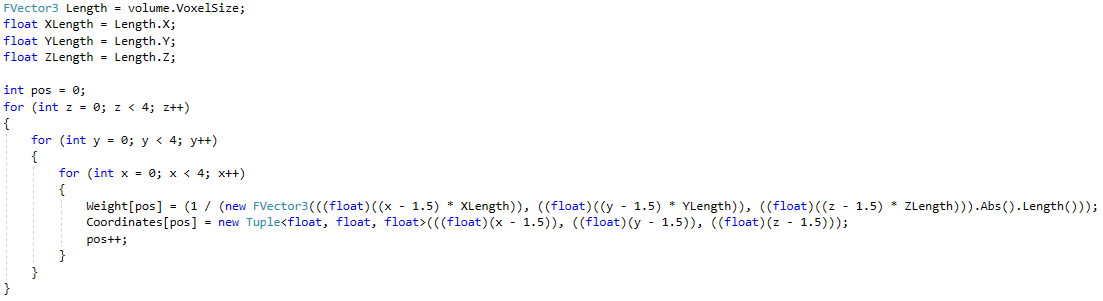
\includegraphics[width=1.2\textwidth]{Logos/Nachbar_Code_Hell_Kurz.PNG}
\caption{Implementierung der Berechnung der Gewichte und Koordinaten} 
\label{fig:gewicht_koord} 
\end{figure}



\begin{figure}[!h] 
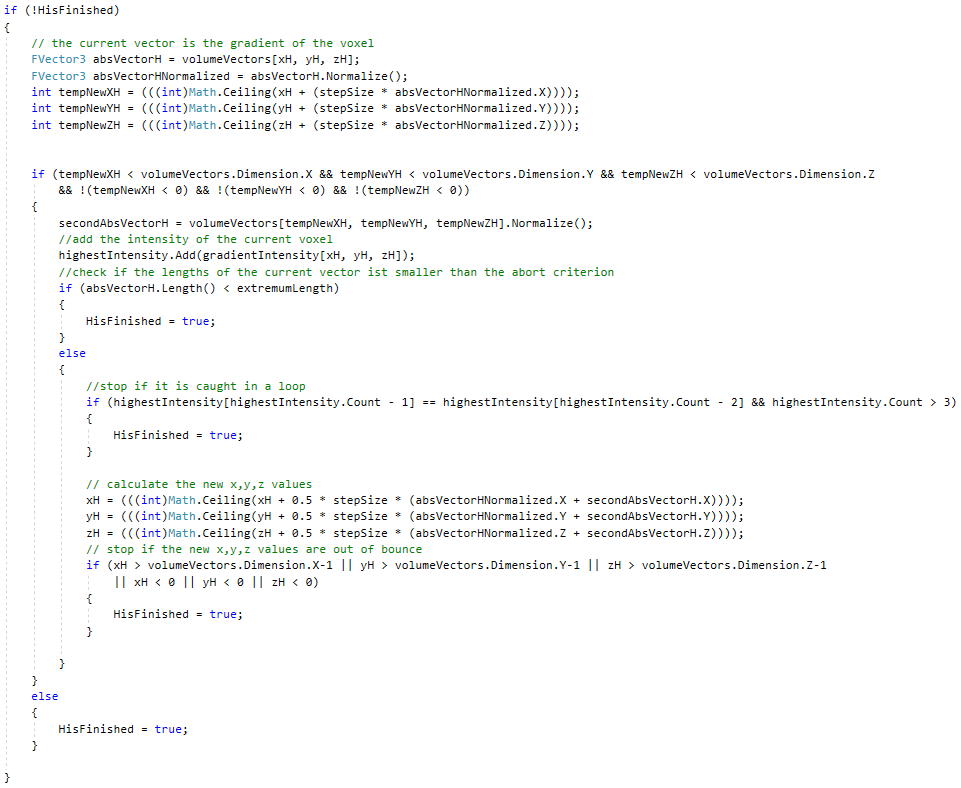
\includegraphics[width=1.2\textwidth]{Logos/LH_Code.PNG}
\caption{Implementierung der Berechnung der High-Werte} 
\label{fig:lh_code} 
\end{figure}


In \autoref{fig:lh_code} kann man den Code zur Berechnung eines High-Wertes sehen. Der Code liegt innerhalb einer while-Schleife, die so lange aufgerufen wird, bis \textit{HisFinished} und \textit{LisFinished} true sind. Die Berechnung des Low-Wertes ist ebenfalls in der Schleife und sieht bis auf die Richtung der neuen \textit{absVector} und \textit{secondAbsVector} gleich aus.
\newline
Am Anfang eines Durchlaufes wird der normalisierte Gradienten des aktuellen Punktes in \textit{absVectorNormalized} gespeichert. Anschließend wird der Punkt des zweiten normalisierten Vektors berechnet. Liegt dieser außerhalb des Volumens, so wird die Integration beendet. und der Wert des letzten besuchten Voxels als Ergebnis zurückgegeben, da das Ergebnis immer der letzte Eintrag der Liste \textit{highestIntensity} ist. Liegt er jedoch innerhalb des Volumens, so wird der \textit{secondAbsVector} berechnet und der Intensitätswert des aktuellen Punktes zu der Liste hinzugefügt. Ist der Gradient des aktuellen Punktes kleiner als \textit{extremumLength}, was im Falle von CT-Daten bei null liegt, wird die Integration beendet. Andernfalls wird der neue Punkt mithilfe von \textit{absVectorNormalized} und \textit{secondAbsVecotr} gemäß Hong's Verfahren \cite{hong2003method} ermittelt. Erneut endet die Integration, falls dieser Punkt außerhalb des Volumens liegt. Vor der Berechnung des nächsten Punktes, wird jedoch über die \textit{highestIntensity} Liste nach Schleifen gesucht. Bei sehr kleinen Gradienten, die jedoch größer als null sind, kann es vorkommen, dass das Verfahren immer wieder den selben Punkt findet und somit in einer Endlosschleife feststeckt. Diese Kontrolle könnte jedoch über die Koordinaten der iterierten Punkte geschehen, um dem unwahrscheinlichem Fall, dass zwei durch die Integration hintereinander gefundenen Punkte genau den selben Intensitätswert haben.
\newline
Dieser Vorgang wiederholt sich für den High- als auch für den Low-Wert solange, bis die Integration aus einem der gegebenen Abbruchkriterien stoppt. Es wurde jedoch, um die Anzahl an Clustern übersichtlich zu halten und unbedeutende kleine Cluster auszusortieren eine Mindestgröße der Cluster von 1000 Elementen eingeführt.



Die Implementierung des LH-Clusterings wurde mit einer parallelen For-Schleife realisiert, die über die L-Werte mit der gegebenen Schrittweite von 5 iteriert. Für jede Spalte i wird dann, die in \autoref{alg:clustering} beschriebene Funktion aufgerufen. Die erste For-Schleife beginnt bei i, aus dem Grund, dass es im LH-Histogramm keine Einträge gibt, bei denen der Low- höher als der High-Wert ist, und wird mit der selben Schrittweite hochgezählt. Das Clustern passiert für jeden Punkt $(i, j)$. Der Temporäre Cluster, der alle dazugehörigen Punkte speichert, speichert lediglich die Information welcher Punkt im Histogramm zum Cluster gehört, jedoch nicht die räumlichen Informationen der Punkte. Erst am Ende der parallelen Schleife, wenn alle Ergebnisse gesammelt und die Cluster verschmolzen wurden, werden die Daten ausgelesen.

\IncMargin{1em}
\begin{algorithm}
\SetKwData{Left}{left}\SetKwData{This}{this}\SetKwData{Up}{up}
\SetKwFunction{Union}{Union}\SetKwFunction{FindCompress}{FindCompress}
\SetKwInOut{Input}{input}\SetKwInOut{Output}{output}

 \Input{LH-Histogramm, Spalte i}
 \Output{LH-Clusters}
 \BlankLine
 $AlleErgbnisCluster$\;
 $NeuerMittelpunkt$\;
 $AlterMittelpunkt$\;
 $AktuellerCluster$\;
 \For{$j\leftarrow i$ \KwTo Rand des Histogramms, Schrittweite: 5}{
  $Mittelpunkt \leftarrow (i,j)$\;
 \While{Abstand(NeuerMittelpunkt, AlterMittelpunkt) > Threshold}{
  \For{$(k, l)\leftarrow$ Alle Punkte im Radius der Bandbreite um den Mittelpunkt}{
    \If{IstInReichweiteVomMittelpunkt((k, l))}{
      \If{NochNichtTeilDesClusters((k, l))}{
	$AktuellerCluster.Hinzufügen((k, l))$\;
     }
    }
    $NeuerMittelpunkt \leftarrow NeuenMittelpunktBerechnen(AktuellerCluster)$\;
   }
  }
  $AlleErgebnisCluster.Hinzufügen(AktuellerCluster)$\;
 $ Leeren(AktuellerCluster)$\;
 }
$VerschmelzeNaheCluster(AlleErgebnisCluster)$\;
$return AlleErgebnisCluste$r\;

 \caption{Pseudocode der Implementierung der LH-Cluster}
 \label{alg:clustering}
\end{algorithm}\DecMargin{1em}






Das LH-Clustering wurde anfangs wie im Paper von Nguyen \cite{nguyen2012clustering} über das gesamte Histogramm mit einer Bandweite von 7\% des maximalen LH-Wertes für jeden Kasten berechnet. Dies ist aus mehreren Gründen schlecht. Zum einen ist der maximale LH-Wert sehr hoch, über 4000, obwohl in etwa nur 0,3\% Voxel einen Wert von über 2400 haben. Zum anderen liegen über 5\% der LH-Werte unter 5. Die Kombination aus diesen Gründen, machte das Clustering extrem langsam. Im Bereich von 0 bis 50  wurde in einem sehr großen Radius geclustert, wodurch mit jeder Iteration sehe viele Cluster gefunden und hinzugefügt werden mussten. Eine erste Maßnahme um das Problem zu beheben, war es alle Low- und High- Werten, die über 2400 waren jeweils auf 2400 zu setzten. Dadurch wurden nur wenige Werte verändert und der Clusteringradius wurde deutlich kleiner. Dies konnte das beschriebene Problem jedoch nicht alleine lösen, da immer noch viele Punkte gefunden und dies für jeden Kasten im Histogramm durchgeführt werden musste. Also wurde als nächste Verbesserung eine Schrittweite beim Clustern eingeführt, dies geschah aus der Beobachtung heraus, dass zwei bis drei oder eventuell sogar mehr direkt nebeneinanderliegende Kasten meist zum selben oder einen so ähnlichen Cluster führen, dass diese im letzten Schritt des Clusteringsverfahrens verschmolzen wurden. Diese Änderung verbesserte die Berechnungszeit erneut, jedoch  dauert die Berechnung immer noch relativ lange und es entstanden sehr viele Cluster. Diese durchzuschauen benötigte viel Zeit und das Gehirn wurde meist als viele sehr große Cluster erkannt. Daraufhin wurde das Clustering auf einen LH-Wertbereich von 1025 bis 1075 begrenzt und die Bandweite auf 0,1\% des maximalen LH-Wertes gesetzt. Diese Änderung führte zum Erfolg und das Ventrikelsystem war innerhalb der paar hunderten Clustern mit ein bisschen Aufwand zu erkennen.


Das räumliche Clustern stellte wenig Probleme dar, da die Implementierung des vorigen Schrittes mit der Änderung vom zweidimensionalen Histogramm zum dreidimensionalem Raum übernommen werden konnte.































































